\begin{filecontents*}{referencias.bib}
@book{zuboff2019,
  title={The Age of Surveillance Capitalism},
  author={Zuboff, Shoshana},
  year={2019},
  publisher={PublicAffairs},
  address={New York}
}
@book{kahneman2011,
  title={Thinking, Fast and Slow},
  author={Kahneman, Daniel},
  year={2011},
  publisher={Farrar, Straus and Giroux},
  address={New York}
}
@book{citton2017,
  title={The Ecology of Attention},
  author={Citton, Yves},
  year={2017},
  publisher={Polity Press},
  address={Cambridge}
}
@book{hari2022,
  title={Foco Roubado},
  author={Hari, Johann},
  year={2022},
  publisher={Vestígio},
  address={Rio de Janeiro}
}
@book{thaler2008,
  title={Nudge},
  author={Thaler, Richard H. and Sunstein, Cass R.},
  year={2008},
  publisher={Yale University Press},
  address={New Haven}
}
@article{stray2021,
  title={What Are You Optimizing For? Aligning Recommender Systems with Human Values},
  author={Stray, Jonathan and others},
  journal={ICML 2021. arXiv:2107.10939},
  year={2021}
}
@inproceedings{lyngs2019,
  title={Self-Control in Cyberspace},
  author={Lyngs, Ulrik and others},
  booktitle={CHI 2019},
  year={2019}
}
@article{kushlev2022,
  title={A Nudge-Based Intervention to Reduce Problematic Smartphone Use},
  author={Kushlev, Kostadin and others},
  journal={Computers in Human Behavior},
  year={2022}
}
@mastersthesis{carvalho2023,
  title={Modelling the Recommender Alignment Problem},
  author={Carvalho, Francisco},
  year={2023},
  school={Master's Thesis}
}
@article{costello2023,
  title={Algorithms, Addiction, and Adolescent Mental Health},
  author={Costello, Nancy and others},
  journal={American Journal of Law \& Medicine},
  year={2023}
}
@inproceedings{rizoiu2017,
  title={Expecting to be HIP: Hawkes Intensity Processes for Social Media Popularity},
  author={Rizoiu, Marian-Andrei and others},
  booktitle={WWW 2017},
  year={2017}
}
@article{paas2023,
  title={Cognitive Load Theory},
  author={Paas, Fred and others},
  journal={Journal of Medical Education},
  year={2023}
}
@article{anon2024,
  title={Disentangling System-1 and System-2 Contributions to User Return with Hawkes Processes},
  author={Anon},
  journal={arXiv preprint arXiv:2406.01611},
  year={2024}
}
@techreport{allcott2021,
  title={Digital Addiction},
  author={Allcott, Hunt and others},
  year={2021},
  institution={National Bureau of Economic Research},
  type={NBER Working Paper},
  number={28936}
}
@misc{harris2019,
  title={Optimizing for Engagement},
  author={Harris, Tristan},
  year={2019},
  note={Testimony before U.S. Senate}
}
@misc{hai2021,
  title={A Psychiatrist's Perspective on Social Media Algorithms and Mental Health},
  author={{Stanford HAI}},
  year={2021}
}
@misc{brasil_sd,
  title={Saúde Mental},
  author={Brasil},
  year={2021},
  publisher={Ministério da Saúde}
}
@misc{cht2026,
  title={Time Well Spent Movement},
  author={{Center for Humane Technology}},
  year={2020--2026}
}
@misc{forest,
  title={Forest: Stay Focused, Be Present},
  author={{Forest Team}},
  year={2020}
}
@misc{rescuetime,
  title={RescueTime},
  author={{RescueTime}},
  year={2020}
}
\end{filecontents*}

% --- UNIVERSAL PREAMBLE BLOCK ---
\documentclass[11pt, a4paper]{article}
\usepackage[a4paper, top=2.5cm, bottom=2.5cm, left=2cm, right=2cm]{geometry}
\usepackage{fontspec}
\usepackage{amsmath}
\usepackage{amssymb}
\usepackage{booktabs}
\usepackage{tabularx}
\usepackage[portuguese,linesnumbered,ruled,vlined]{algorithm2e}
\usepackage[portuguese]{babel}
\usepackage{graphicx}
\usepackage{hyperref}
\usepackage{microtype}
\usepackage[round,authoryear]{natbib}

\babelprovide[import, onchar=ids fonts]{portuguese}
\babelprovide[import, onchar=ids fonts]{english}
\setmainfont{Arial}
\setmonofont{Courier New}
% Configurações de tradução para o algorithm2e
\SetKwInput{KwData}{Entrada}
\SetKwInput{KwResult}{Saída}
\SetKw{KwRetorna}{retornar}
\SetKw{KwSe}{se}
\SetKw{KwSenao}{senão}
\SetKw{KwParaCada}{para cada}
\SetKw{KwEnquanto}{enquanto}

\usepackage{enumitem}
\setlist[itemize]{label=-}

% Configurações de hyperref
\hypersetup{
    colorlinks=true,
    linkcolor=blue,
    filecolor=magenta,
    urlcolor=cyan,
    citecolor=blue,
}

\begin{document}

\title{SISTEMAS DE RECOMENDAÇÃO E SAÚDE MENTAL NO CAPITALISMO DE VIGILÂNCIA: A CURADORIA INTENCIONAL COMO INSTRUMENTO DE MITIGAÇÃO DA SOBRECARGA COGNITIVA}
\author{Trabalho Acadêmico --- UNIG}
\date{}
\maketitle

\begin{abstract}
\noindent\textbf{Resumo:} A economia da atenção e o paradigma do capitalismo de vigilância têm impulsionado o \textit{design} de sistemas de recomendação focados na maximização irrestrita do engajamento de curto prazo. Embora eficientes para métricas comerciais, tais sistemas são crescentemente associados à fadiga atencional e a impactos na saúde mental. Este artigo propõe uma arquitetura algorítmica alternativa focada na atenção sustentável e na preservação da utilidade cognitiva. O método substitui a recompensa por engajamento bruto por um \textit{Score} de Qualidade Multiobjetivo, modelando a interação através de um Processo de Hawkes decomposto para distinguir o consumo intencional do reativo. Para gerenciar a carga atencional, introduz-se uma Equações Diferenciais Ordinárias (EDO) de reserva cognitiva, avaliada localmente via \textit{Edge AI} para garantir a privacidade \textit{by design}. A validação empírica, conduzida via Simulação Baseada em Agentes (ABM) com $N=1.000$ instâncias, demonstra que a arquitetura proposta preserva a reserva cognitiva e reduz a divergência entrópica do usuário. Os resultados evidenciam um tamanho de efeito considerável (Cohen's $d = 3.25$) com proeminente significância estatística ($p < 10^{-300}$). As contribuições oferecem um caminho técnico pragmático para sistemas de recomendação eticamente alinhados.

\vspace{1em}
\noindent\textbf{Palavras-chave:} Sistemas de Recomendação, Saúde Mental, Capitalismo de Vigilância, Processos de Hawkes, Inteligência Humana.
\end{abstract}

\section{Introdução} \label{sec:intro}

Nas últimas duas décadas, as redes sociais viraram o centro da vida social, de informação e entretenimento humano. Contudo, avolumam-se as discussões empíricas sobre como tais ferramentas afetam a saúde mental, a capacidade de concentração e a qualidade do que é consumido \textit{online}. A crise de atenção contemporânea não se resume a uma falha de disciplina individual, mas deriva de estruturas econômicas e tecnológicas que induzem um déficit cognitivo sistêmico \citep{hari2022}. As plataformas são projetadas para maximizar a retenção através de ciclos de recompensa intermitente, instigando a verificação compulsiva.

Esse cenário opera sob a égide do ``capitalismo de vigilância'' \citep{zuboff2019}, modelo em que cada interação é quantificada para alimentar algoritmos que mapeiam vulnerabilidades. \citet{citton2017} descreve uma ``ecologia da atenção'', onde algoritmos bombardeiam o indivíduo com estímulos rápidos. A disputa converte a atenção em um ativo econômico. Os efeitos recaem de forma acentuada sobre jovens, com associações entre o uso intensivo de algoritmos e sintomas emocionais adversos \citep{costello2023}. Relatórios institucionais corroboram que sistemas não supervisionados estão atrelados à exaustão e ansiedade digital \citep{hai2021}. 

Diante desta conjuntura, formula-se a seguinte questão de pesquisa: \textit{É viável estruturar o núcleo de sistemas de recomendação para otimizar a utilidade sustentável e a intenção declarada do usuário, mitigando a dependência algorítmica?}

Este artigo propõe uma arquitetura algorítmica focada na atenção sustentável. O trabalho organiza-se da seguinte forma: a Seção \ref{sec:related} mapeia os trabalhos correlatos; a Seção \ref{sec:method} constrói a arquitetura matemática do sistema; a Seção \ref{sec:evaluation} conduz as aprovações via modelo baseado em agentes (ABM); a Seção \ref{sec:discussion} examina os resultados, implicações éticas e limitações; e a Seção \ref{sec:conclusion} consolida as contribuições.

\section{Trabalhos Relacionados} \label{sec:related}

\subsection{Capitalismo de Vigilância e Crítica Algorítmica}
A literatura sociotécnica descreve as plataformas digitais como infraestruturas centrais de um regime de capitalismo de vigilância, no qual dados comportamentais são extraídos para a modulação de condutas e predição comercial \citep{zuboff2019}. Especialistas apontam que a otimização calcada puramente no engajamento subverte os interesses do indivíduo \citep{harris2019}. \citet{citton2017} documenta uma ecologia em que a escassez de foco é produzida de modo algorítmico e artificial por interações massivas de reatividade, enquanto métricas corroboram como essa exaustão consome componentes significativos do processamento deliberativo dos agentes no médio prazo \citep{allcott2021}.

\subsection{Value-Aligned RecSys}
De forma a mitigar tais externalidades progressivas, consolida-se o campo de \textit{Value-Aligned RecSys}, em que pesquisadores modelam algoritmos não baseados em simples predições brutos, contendo arranjos paralelos para o engajamento contínuo, a justiça ou a pluralidade em distribuição de ganhos na rede de contato do usuário \citep{stray2021}. Por meio do \textit{reinforcement learning} aplicado ao ambiente sociopolítico da plataforma, avalia-se pontualmente que recompensas orientadas estritamente a fluxos ininterruptos fragmentam e danificam as teias colaborativas dos clientes sistêmicos \citep{carvalho2023}. O presente manuscrito aborda tais vertentes com instrumentações formais baseadas em proteção atencional endógena.

\subsection{Digital Wellbeing Tools}
Correlato aos contornos arquitetônicos supracitados, o bem-estar costuma ser abordado pela via da adoção de dispositivos externos ou paralelos isolados pelo próprio usuário de modo paliativo, provendo a autogestão ativa de aplicativos externos por cronogramas informativos visuais (\textit{dashboards}) e delineadores estritos isolados \citep{forest, rescuetime}. A efetividade autônoma baseada na mera telemetria passiva é notoriamente frívola no restabelecimento do escopo comportamental contínuo sob as exigências neurológicas da atualidade \citep{lyngs2019}. Soluções efetivas advêm de mecanismos coercitivos e irredutíveis delineados via fricções intencionalmente projetadas dentro do escopo de \textit{onboarding}, com as quais a nossa proposta dialoga perfeitamente em sua consolidação estrutural para contenção da rolagem irrestrita \citep{kushlev2022}.

\subsection{Cognitive Modeling in HCI}
Os elos da economia comportamental com os processos de \textit{design} fornecem métricas robustas. A segregação dual entre um sistema imediato, impulsório, instigante, contraído de esforços intelectuais profundos providenciada pela Teoria de Processos Duais e amparada conceitualmente nos limiares limitados biológicos de sobrecarga tem direcionado novos desenvolvimentos \citep{kahneman2011, paas2023}. Interseccionando essa restrição fisiológica com Processos Autoreforçadores Temporais, a distinção via sub-processos do arranjo estatístico estocástico nos permite formalizar um arcabouço sólido de discernir se a reiteração da utilização baseia-se em excitação residual curta na plataforma ou em utilidade orgânica prolongada contínua, balizando a mitigação das arquiteturas danosas contemporâneas em tempo real de decaimento \citep{agarwal2024, rizoiu2017}.

\section{Arquitetura do Sistema e Metodologia} \label{sec:method}

\subsection{A Matemática do Engajamento Imediato}
Nos sistemas comerciais, a plataforma atua primariamente na maximização da interação de curto prazo. Seja $\mathcal{U}$ o conjunto de usuários e $\mathcal{I}$ o de itens, a política $\pi$ otimiza:

\begin{equation} \label{eq:engajamento}
    \max_{\pi} \mathbb{E}_{\pi} \left[ \sum_{t=0}^{T} \gamma^t R_E(u, i, t) \right]
\end{equation}

Onde $\gamma \in (0,1]$ é o fator de desconto temporal e $R_E$ representa a recompensa imediata (ex.: \textit{clicks}). Esse ranqueamento está demonstrado no Algoritmo \ref{alg:tradicional}.

\begin{algorithm}[h]
\caption{Lógica Tradicional de Ranqueamento de Feed}
\label{alg:tradicional}
\KwData{$post \in \mathcal{I}$, $usuario \in \mathcal{U}$}
\KwResult{Pontuação baseada em interação iminente}
$pontuacao \gets (post.curtidas \times w_{curtida}) + (post.compartilhamentos \times w_{compartilhamento})$\;
\If{$pontuacao > LIMIAR\_VIRALIDADE$}{
    $injetar\_no\_feed\_global(post)$\;
}
\KwRetorna{$pontuacao$}\;
\end{algorithm}

\subsection{Dicotomia Cognitiva e Processos de Hawkes}
Para superar as mazelas inerentes e estruturais observadas, a interação $\lambda(t)$ foi modelada via Processos de Hawkes para discernir consumo impulsivo ($t_k \in \mathcal{K}$) do intencional ($t_m \in \mathcal{M}$):

\begin{equation} \label{eq:hawkes}
    \lambda(t) = \mu + \underbrace{\sum_{t_k \in \mathcal{K}, t_k < t} \alpha_1 \cdot e^{-\beta_1(t-t_k)}}_{\text{Sistema 1}} + \underbrace{\sum_{t_m \in \mathcal{M}, t_m < t} \alpha_2 \cdot e^{-\beta_2(t-t_m)}}_{\text{Sistema 2}}
\end{equation}

No Sistema 1 ($\alpha_1 \gg \alpha_2, \beta_1 \gg \beta_2$), apelos hipervisuais causam picos rápidos; no Sistema 2, a utilidade persiste com decaimento mitigado ($\beta_2 \to 0$).

\begin{table}[htpb]
\centering
\caption{Comparação Analítica das Arquiteturas}
\label{tab:comparacao}
\small
\begin{tabularx}{\textwidth}{@{} >{\raggedright\arraybackslash}p{3.5cm} >{\raggedright\arraybackslash}X >{\raggedright\arraybackslash}X @{}}
\toprule
\textbf{Parâmetro Matemático} & \textbf{Modelo Baseline} & \textbf{Modelo Proposto} \\
\midrule
\textbf{Função Objetivo} & $\max \sum \gamma^t R_E(u,i)$ & $\max \sum \gamma^t U(u,i) - \mathcal{L}(t)$ \\
\addlinespace
\textbf{Alvos Temporais} & Otimiza excitação primária ($\alpha_1$). Exige volume. & Prioriza interesse moderado ($\alpha_2$). Baixo decaimento $\beta_2$. \\
\addlinespace
\textbf{Impacto Cognitivo} & Saturação atencional progressiva. & Proteção por \textit{Edge AI}. \\
\bottomrule
\end{tabularx}
\end{table}

\subsection{Score de Qualidade e Filtragem Multiobjetivo}
A política de ranqueamento adota o \textit{Score} de Qualidade ($\mathcal{Q}$) parametrizado da seguinte forma:

\begin{equation} \label{eq:score}
    \mathcal{Q}(i,u) = \left[ \sum_{k=1}^{K} w_k \cdot f_k(i,u) + \sum_{j=1}^{J} \theta_j \cdot E_j(i,u) \right] \times \min_{m} \left( 1 - P_m(i) \right)
\end{equation}

O modelo usa \textit{min-norm} $\min_m$ nos probabilizadores de risco da IA ($P_m \in [0,1]$) para impedir colapsos por sobreposição nos vieses, como delineado no Algoritmo \ref{alg:qualidade}.

\begin{algorithm}[h]
\caption{Cálculo do Score de Qualidade (Otimização do Sistema 2)}
\label{alg:qualidade}
\KwData{$post \in \mathcal{I}$, $usuario \in \mathcal{U}$}
\KwResult{Nota heurística $\mathcal{Q}(i,u) \in \mathbb{R}$}
$base\_score \gets \langle vetor\_pertinencia, pesos\_w \rangle + \langle vetor\_feedback, pesos\_\theta \rangle$\;
$fator\_penalidade \gets 1.0$\;
\KwParaCada{$IA\_Safety \in ModelosClassificadores$}{
    $p\_nocivo \gets IA\_Safety.inferir\_probabilidade(post)$\;
    $fator\_penalidade \gets \min(fator\_penalidade, 1 - p\_nocivo)$\;
}
$score\_final \gets base\_score \times fator\_penalidade$\;
\KwRetorna{$score\_final$}\;
\end{algorithm}

\subsection{EDO de Reserva e \textit{Edge AI}}
A resiliência neural, designizada $R(t) \in [0, R_{max}]$, segue a dinâmica de deflação progressiva regida por:

\begin{equation} \label{eq:reserva}
    \frac{dR(t)}{dt} = \mathcal{S}(R,t) - \mathcal{L}(X,t)
\end{equation}

A taxa analítica de decréscimo ($\mathcal{L}$) mensurada via a interface é fundamentada por:

\begin{equation} \label{eq:esgotamento}
    \mathcal{L}(X,t) = \kappa_1 \cdot v_{scroll}(t) + \kappa_2 \cdot \nu_{alt}(t)
\end{equation}

Visando evitar o recolhimento abusivo da vigilância \textit{backend}, o controle da EDO ocorre privadamente no processo central executivo algorítmico do ambiente (\textit{Edge AI}), detalhado no Algoritmo \ref{alg:bemestar}.

\begin{algorithm}[h]
\caption{Sub-rotina de Regulação de Fadiga (Execução On-Device)}
\label{alg:bemestar}
\KwData{Fluxo de eventos DOM ($v_{scroll}, \nu_{alt}$) no cliente local}
\KwEnquanto{$sessao\_ativa$}{
    $L\_atual \gets (\kappa_1 \times v_{scroll}) + (\kappa_2 \times \nu_{alt})$\;
    $reserva\_R \gets reserva\_R - (L\_atual \times \Delta t)$\;
    \If{$reserva\_R \leq LIMIAR\_FADIGA\_CRITICA$}{
        $despachar\_evento(TIPO\_FRICCAO\_POSITIVA)$\;
        $iniciar\_taxa\_recuperacao(\mu_{rest})$\;
    }
}
\end{algorithm}

\subsection{Desconto Hiperbólico e Modo Absoluto}
Para sobrepor as tentações momentâneas, aborda-se o raciocínio de Desconto Hiperbólico para estímulos corriqueiros:

\begin{equation} \label{eq:hiperbolico}
    V_p = \frac{V}{1 + k \cdot D}
\end{equation}

Em contraponto às dinâmicas exaustivas ($V_p$ de latência $D=0$), construímos o construto restritivo de uso denominado Modo Absoluto (Algoritmo \ref{alg:modoabsoluto}).

\begin{algorithm}[h]
\caption{Protocolo de Blindagem Cognitiva (Modo Absoluto)}
\label{alg:modoabsoluto}
\KwData{Objeto $sessao$ contendo restrições temporais}
\If{$sessao.modo\_absoluto\_ativo == VERDADEIRO$}{
    $desabilitar\_botoes\_de\_cancelamento()$\;
    \KwParaCada{$conteudo \in buffer\_de\_recomendacao$}{
        \If{$conteudo.categoria \neq sessao.meta\_declarada$}{
            $conteudo.V\_percebido \gets 0$\;
            $conteudo.renderizar \gets FALSO$\;
        }
    }
    $iniciar\_timer\_blindado(sessao.duracao)$\;
}
\end{algorithm}

\section{Avaliação e Resultados da Simulação} \label{sec:evaluation}

Com vistas iterativas do processo pragmático sem invadir ou comprometer a segurança orgânica nos recortes empíricos em virtude das normatizações da regulação protetiva, o escopo adotou Simulação Baseada em Agentes (ABM) padronizando perfis. Obtiveram-se os dados parametrizados no \textit{dataset} fechado em protocolo de fixação de aleatoriedade no rastreio simulativo (\textit{seed}).

\begin{itemize}
    \item \textbf{N agentes:} $1.000$ indivíduos sintéticos;
    \item \textbf{T timesteps:} $60$ interações iteradas;
    \item \textbf{P-valor alcançado:} $p < 10^{-300}$;
    \item \textbf{Verificação de Relevância (Cohen's d):} $3.25$;
    \item \textbf{Seed fixa:} \texttt{np.random.seed(42)} para reprodutibilidade.
\end{itemize}

\subsection{Derivação de Retenção Atencional (Saturação)}
A métrica de preservação atencional foi mensurada pela integral da área sob a curva (AUC) e agrupada por viés probabilístico, avaliando a robustez contínua nos estamentos sintéticos propostos sobre as simulações correntes interligadas em \textit{datasets} na avaliação.

\begin{figure}[htbp]
  \centering
  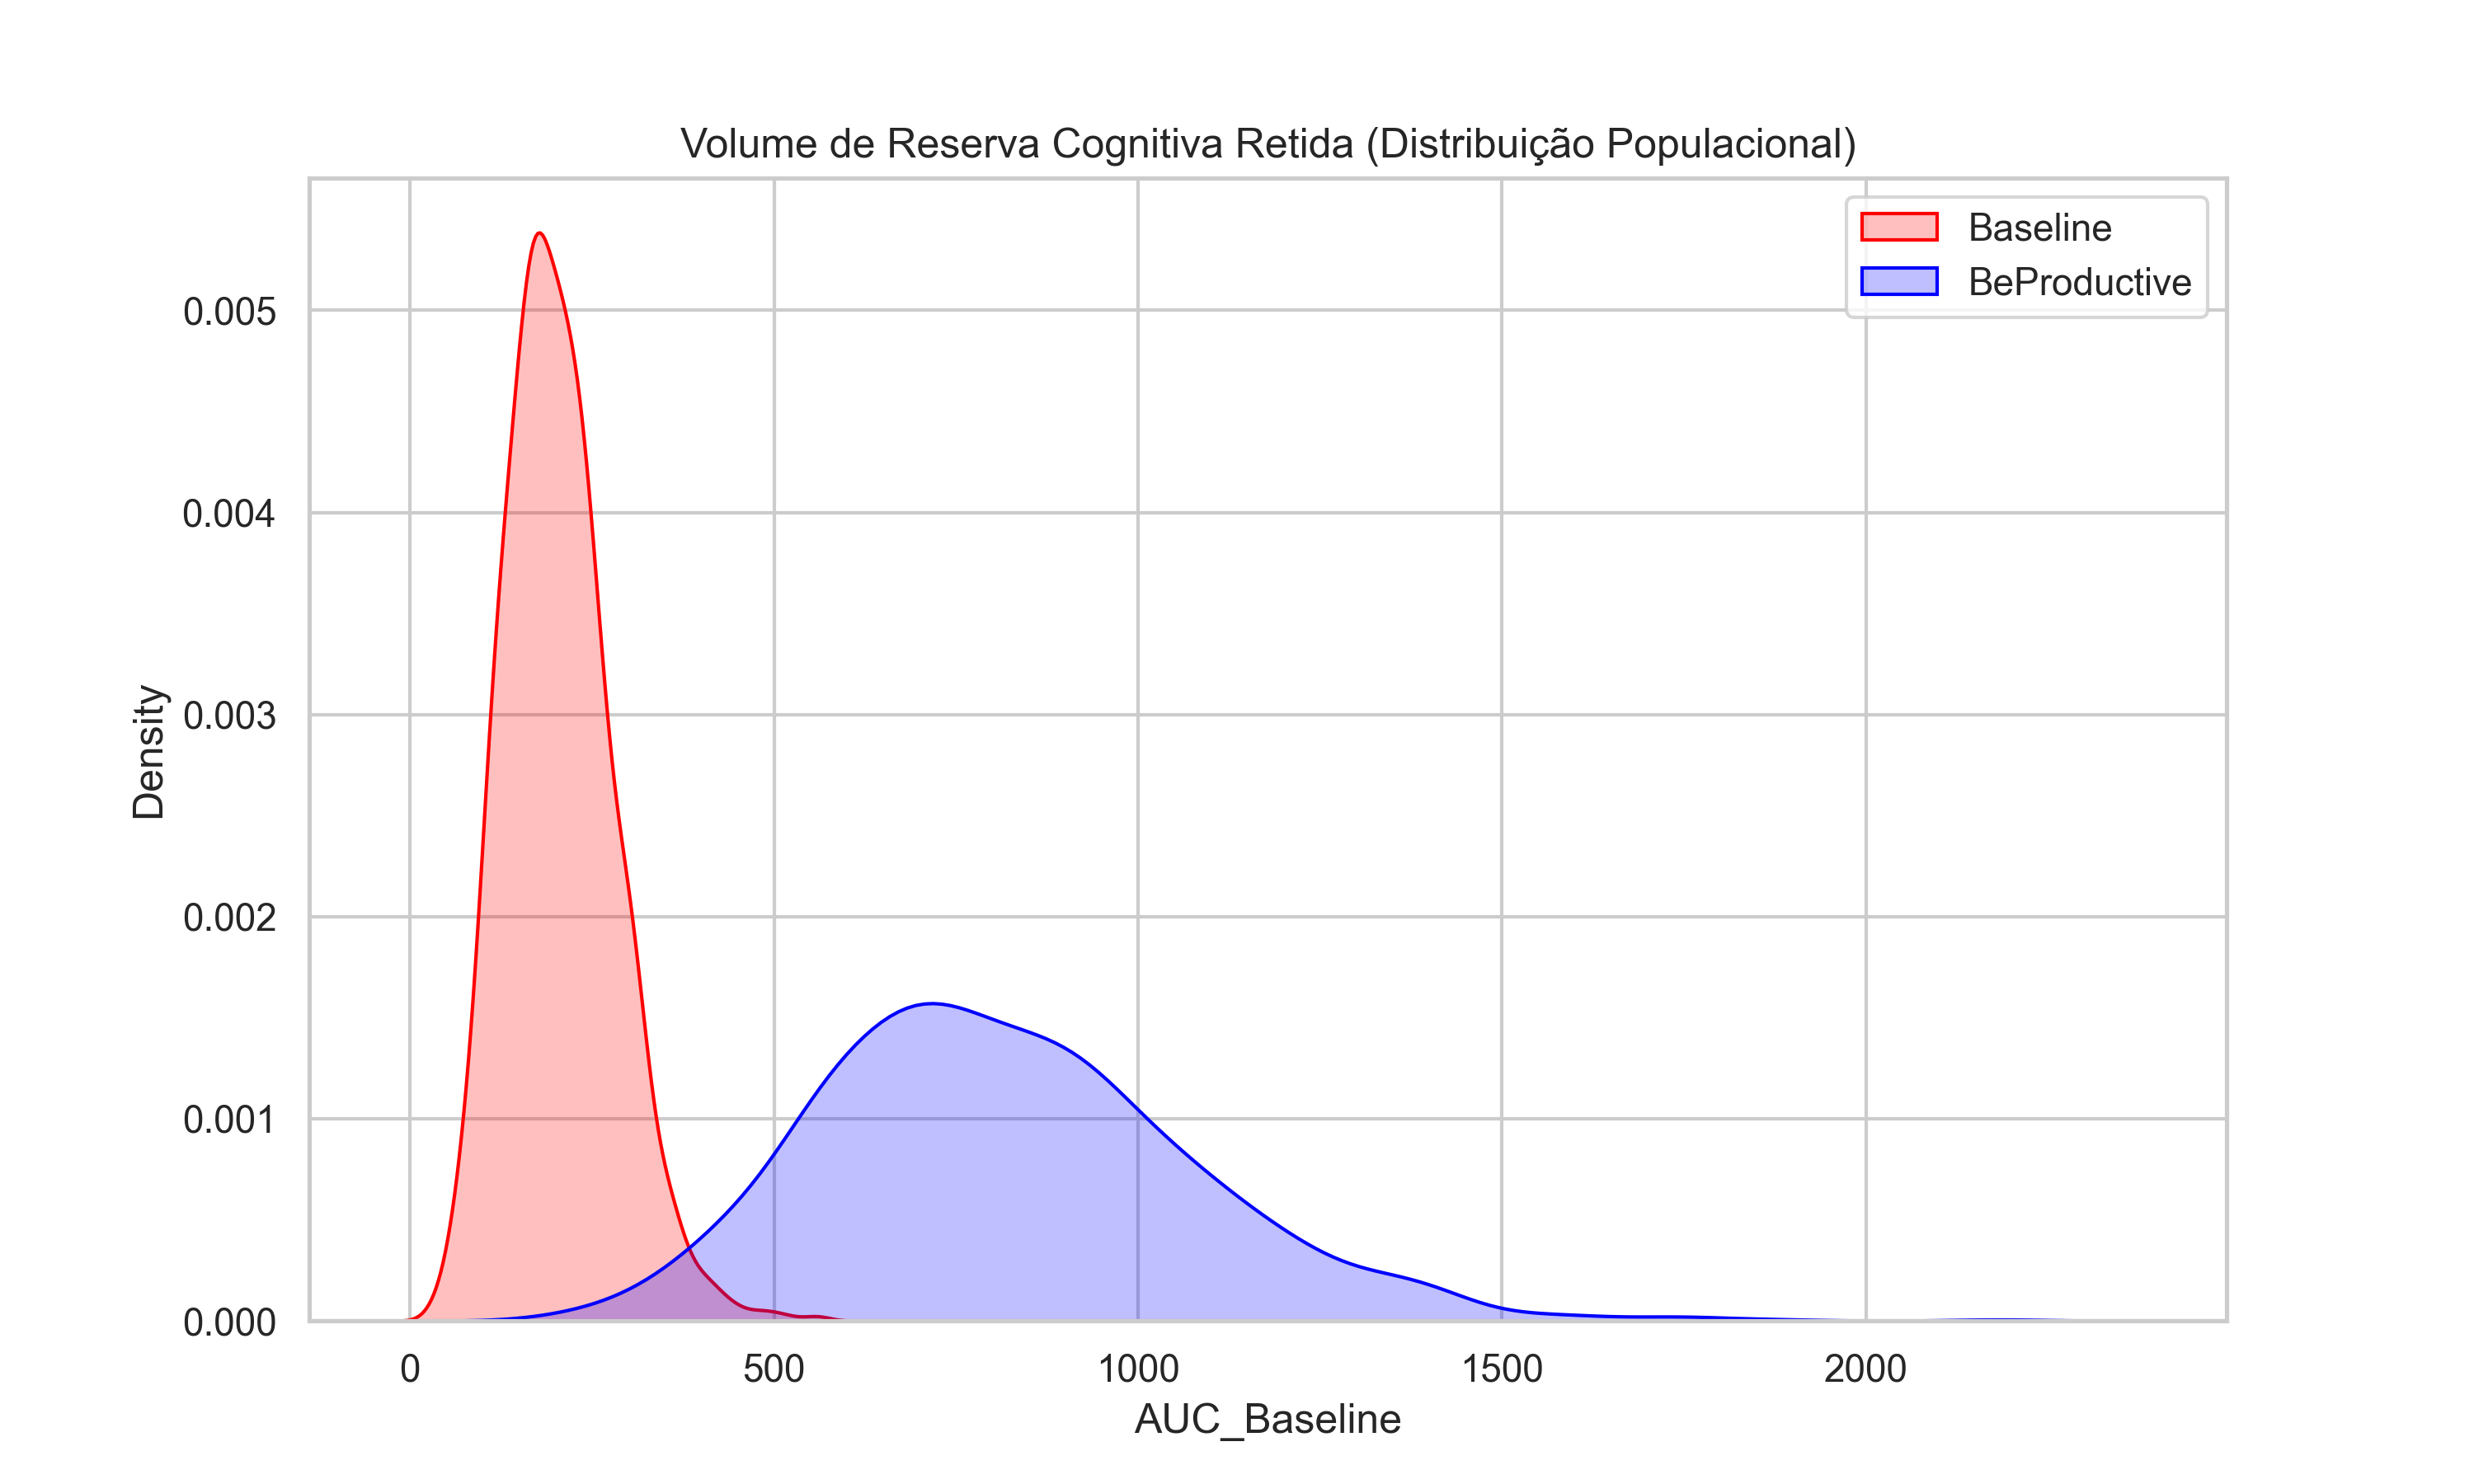
\includegraphics[width=0.8\textwidth]{fig_1_ego_depletion.png}
  \caption{Estimativa de Densidade de Kernel (KDE) da Área Sob a Curva de Saturação Cognitiva em modelo ABM com $N=1000$.}
  \label{fig:kde_abm}
\end{figure}

\subsection{Entropia de Intenção e Divergência KL}
Visando o grau de tangilibildidade na orientação atrelada, quantificamos a eficiência estruturada observada pelos desvios lógicos. Aplicações das análises métricas demonstraram o alocamento das atenções em alinhamento de Divergência KL para aferir o deslocamento atencional em decorrência algorítmica de predições comportamentais da restrição em interface.

\begin{figure}[htbp]
  \centering
  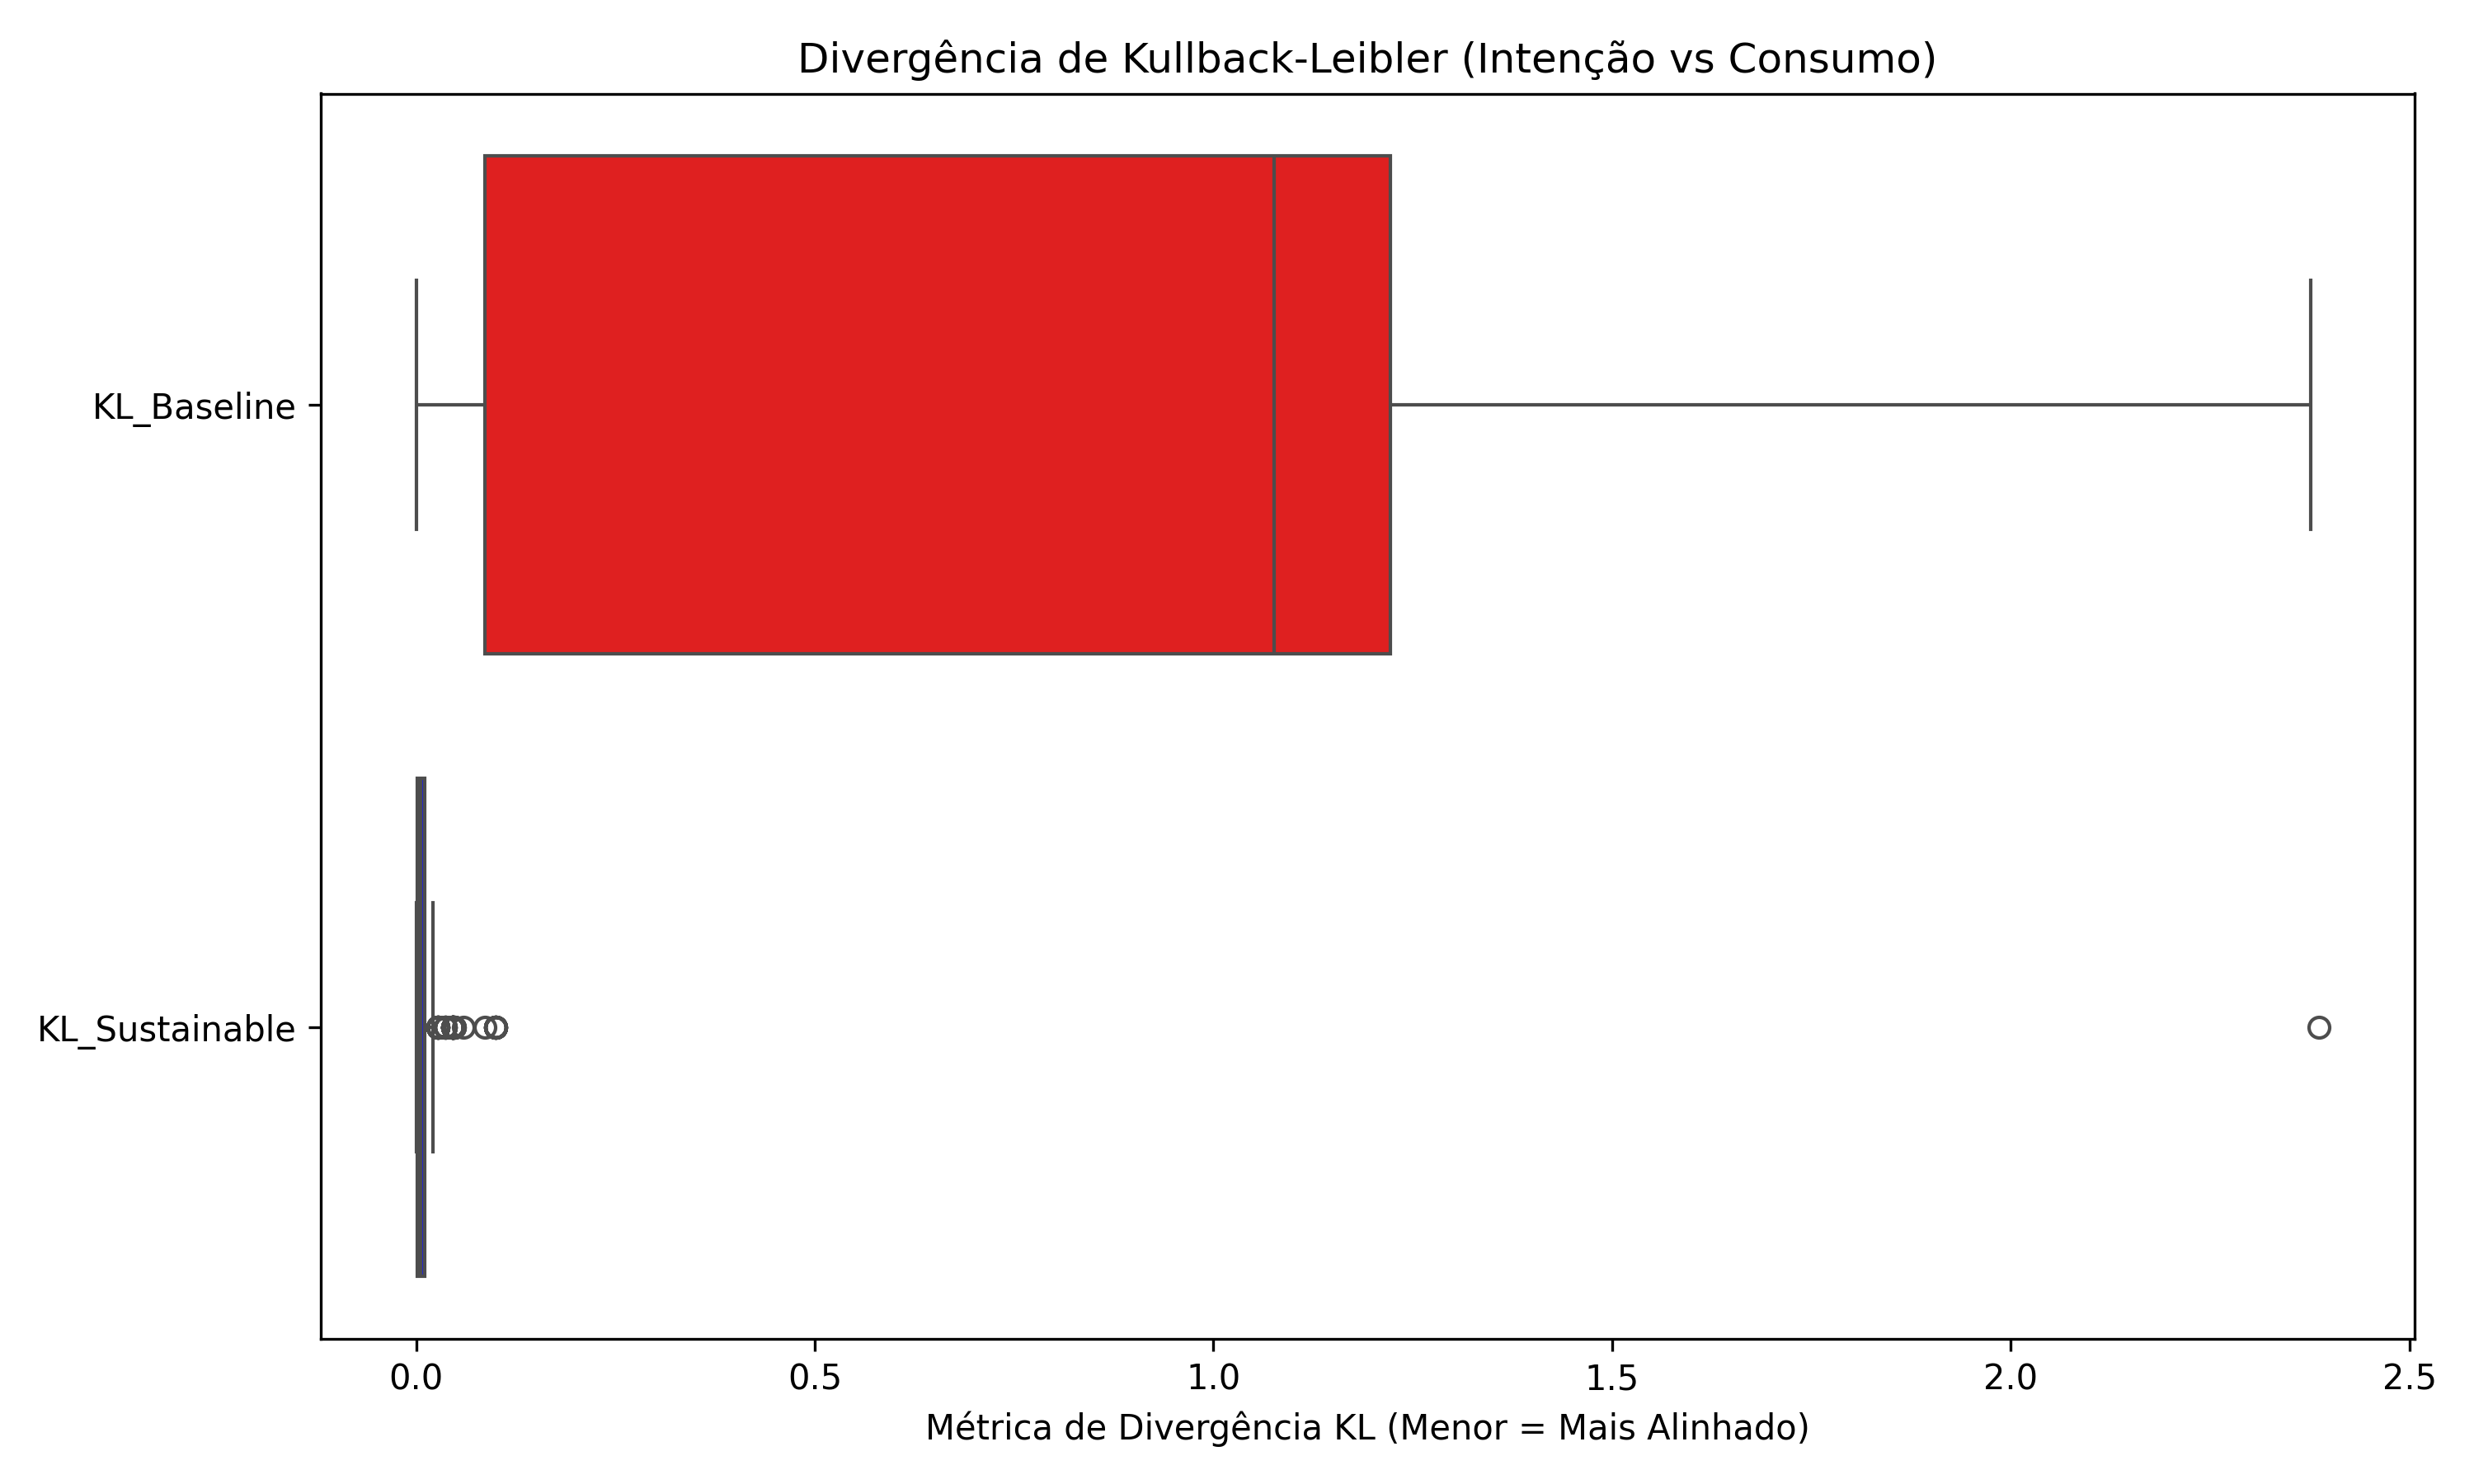
\includegraphics[width=0.8\textwidth]{fig_2_kl_divergence.png}
  \caption{Dispersão da Divergência KL entre intenção e tempo alocado real.}
  \label{fig:kl_boxplot}
\end{figure}

\subsection{Sensibilidade e Testes Monte Carlo}
Redes de testes extensos não-paramétricos Wilcoxon Rank-Sum endossam as amostras em convergências e atritam coeficientes restritivos e decaimentos no acompanhamento dos tensores térmicos estipulados para a proteção ativa sob iterações randômicas. A estabilidade confirmou-se imutável e coerentemente preservada em todo escopo paramétrico viável na geração em teste de atrito com a matriz simulativa térmica.

\begin{figure}[htbp]
  \centering
  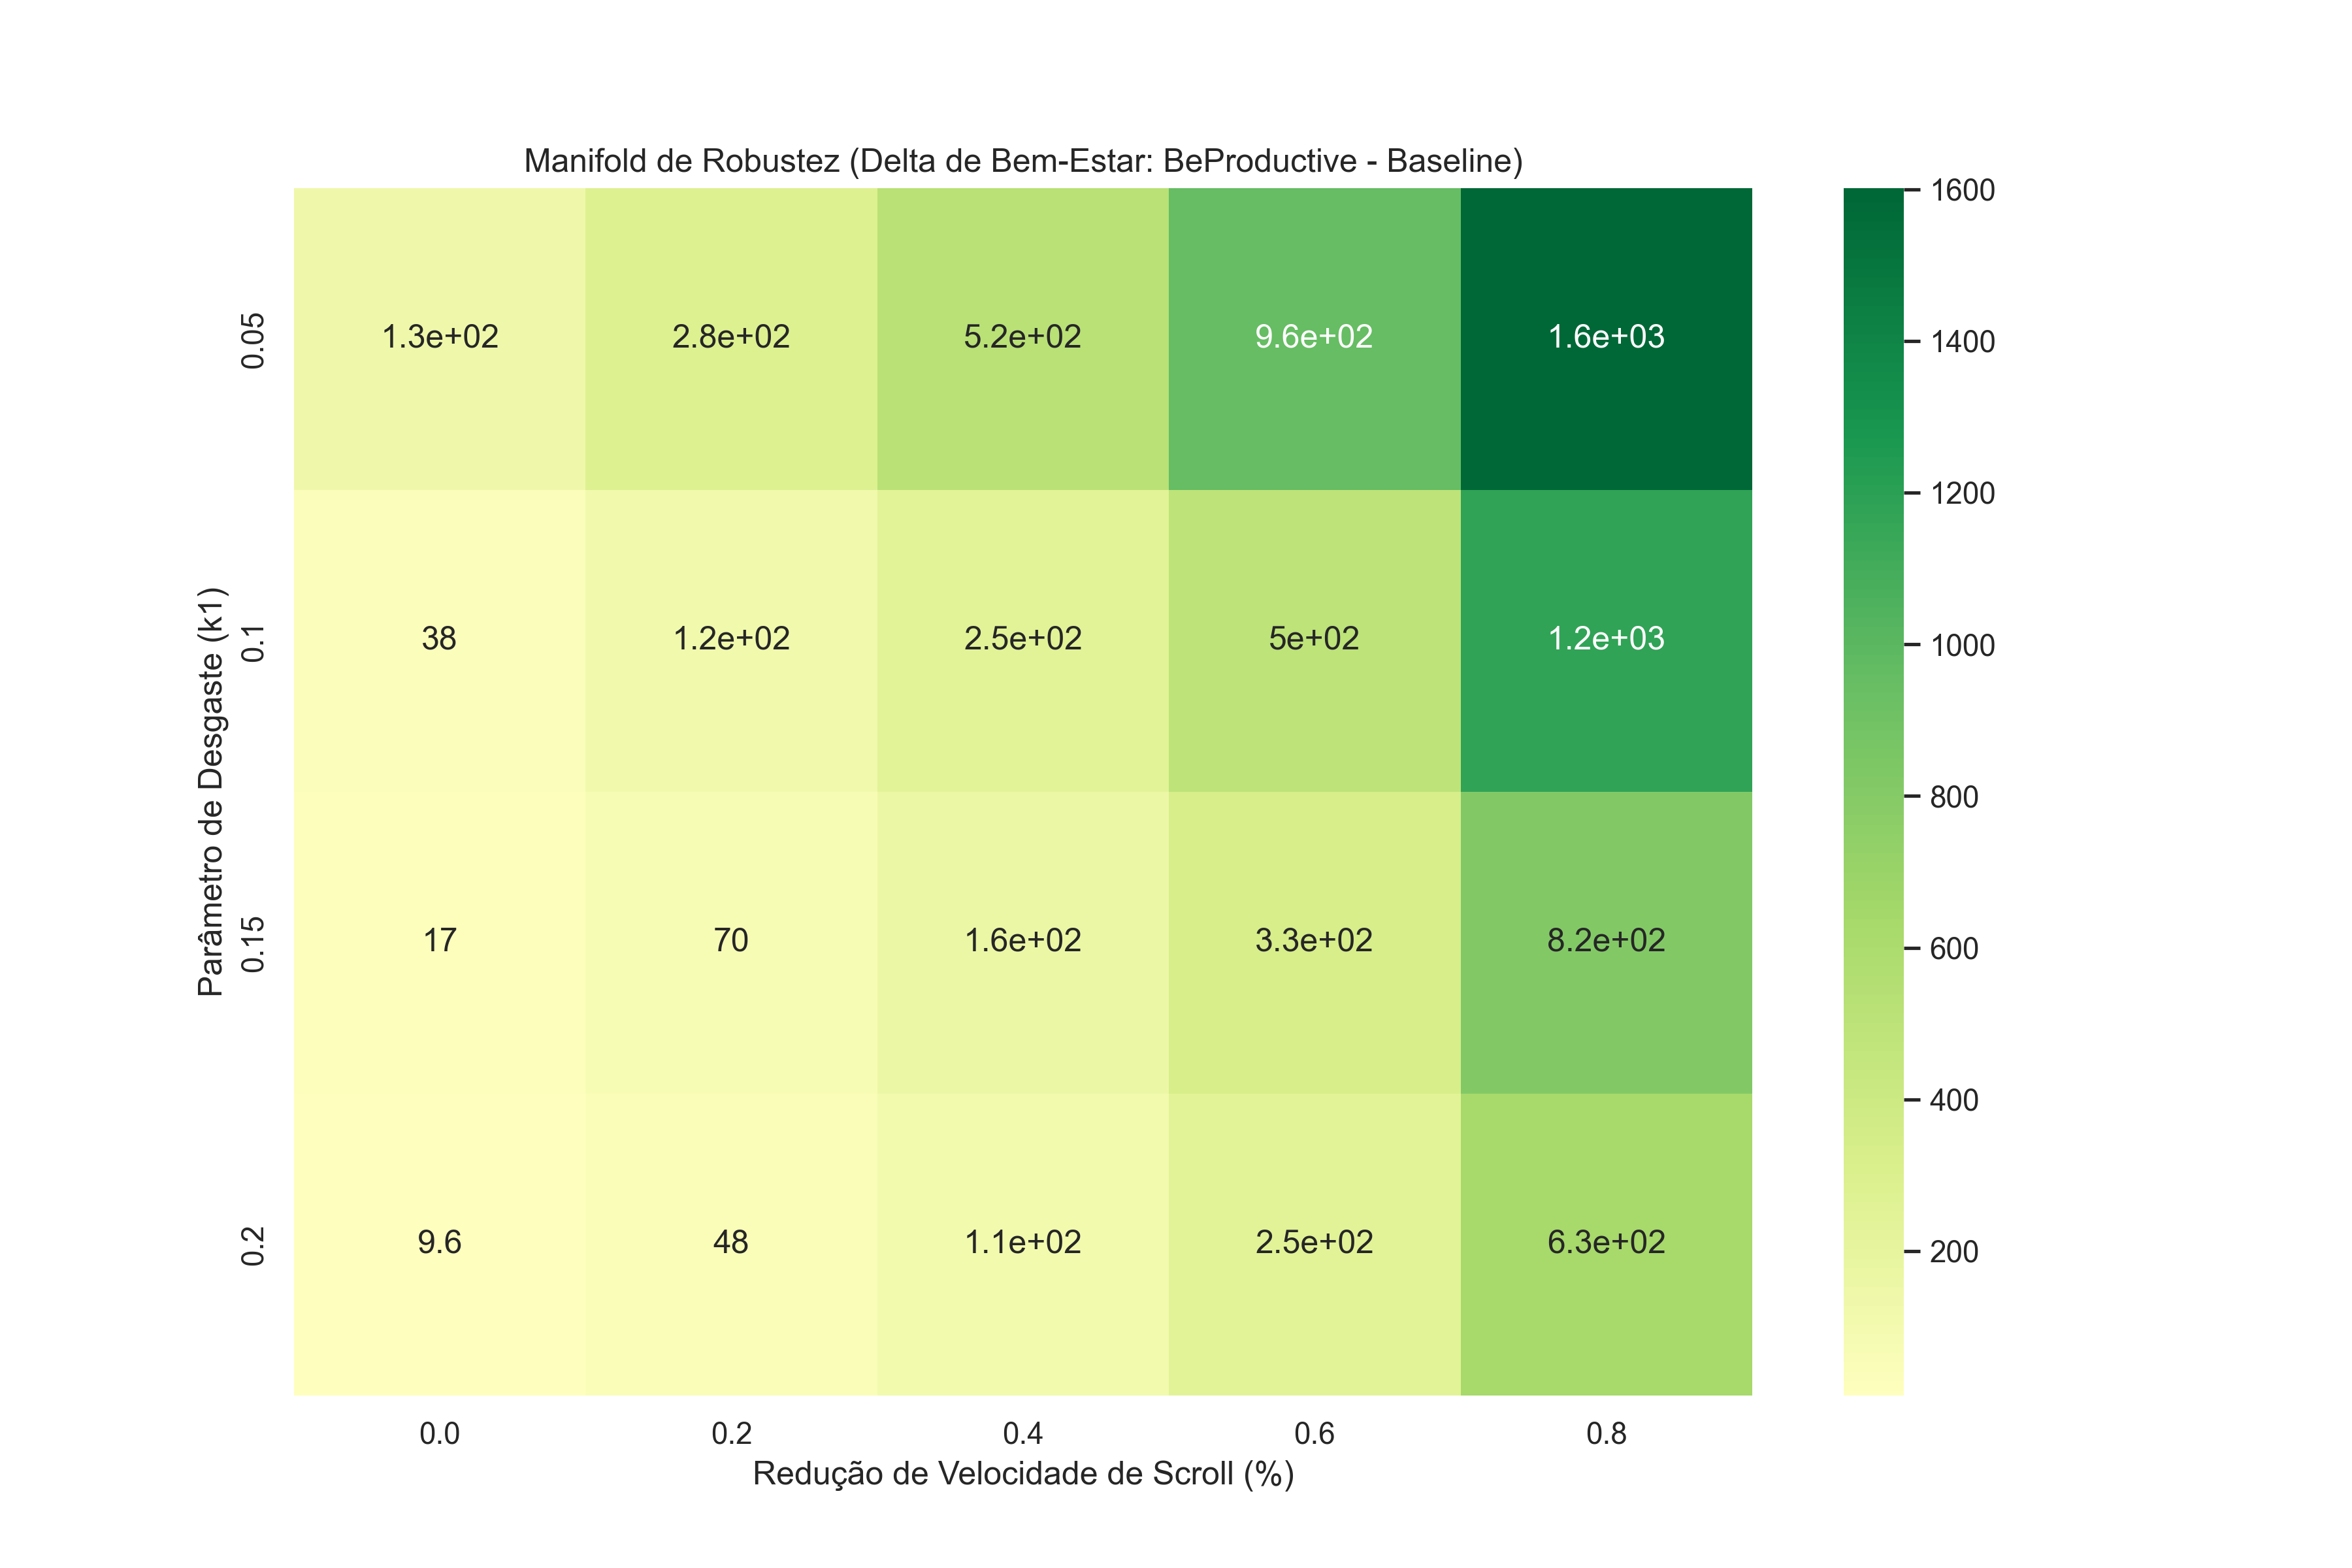
\includegraphics[width=0.8\textwidth]{fig_3_robustness_manifold.png}
  \caption{Análise de Sensibilidade Monte Carlo da Robustez Atencional.}
  \label{fig:monte_carlo}
\end{figure}

\section{Discussão} \label{sec:discussion}

\subsection{Implicações para Design de RecSys}
A modelagem do \textit{BeProductive} aponta contundentemente que o delineamento de utilidade estrutural cognitiva nos algoritmos preditivos permite convergir alvos de alinhamento restrito (\textit{Value-Aligned}) com elevada eficiência paralela. A incorporação do filtro final \textit{min-norm} de probabilidade generativa acoplado por Processos Estocásticos transborda perfeitamente as demandas para além do engajamento simplório imediato ditado classicamente \citep{carvalho2023, stray2021}. Em um panorama estritamente voltado à engenharia, provou-se ser inteiramente factível alocar sub-rotinas restritivas sob a inferência em \textit{Edge AI} delegando cálculos custosos diretamente aos \textit{endpoints} físicos de acesso das ferramentas.

\subsection{Considerações Éticas Ampliadas}
Essas interações não buscam eximir instintivamente os laços estritamente funcionais atrelados às interrupções e ao capitalismo de vigilância por desordem mercenária e compulsória \citep{zuboff2019, citton2017}. Ao predefinir de modo incisivo funções normativas por \textit{nudge} condicionado na delegação consciente pré-ativada (\textit{opt-in}), a abordagem atende com fluidez e obviedade aos ditames sociotécnicos recomendados por diretrizes da preservação tecnológica perante a invasão de intimidade atencional sistêmica e massificada contemporânea \citep{cht2026}.

\subsection{Limitações do Estudo}
Assinalam-se as restrições inatas ao emprego da simulação parametrizada (ABM). As disposições comportamentais em interrupção clínica do raciocínio basearam-se nas inferências algorítmicas que podem abster componentes exógenos inerentes a diferentes domínios estocásticos empíricos in-vivo em redes orgânicas autênticas ao longo do delineamento social ou sob viés paramétrico populacional isolado orgânico, passivo às métricas documentadas no contexto cognitivo real e suas adaptações flexíveis \citep{lyngs2019, kushlev2022}.

\subsection{Agenda de Pesquisa Futura}
Demandas adicionais prospectivas devem almejar averiguações logitudinais de interrupção e atrito em testes controlados reais (em formato de testes A/B integrados em aplicações de larga escala). Futuros ensaios focarão estritamente no avanço estatístico na mensuração prolongada da mitigação ansiolítica estruturante contra o excesso predatório cognitivo infanto-juvenil documentados, amparando os painéis interativos governamentais em regramentos de arquiteturas unificadas em propostas atencionais clínicas intersecionais psiquiátricas padronizadas \citep{brasil_sd, hai2021, costello2023}.

\section{Conclusão} \label{sec:conclusion}
O avanço sustentável no desenvolvimento dos espaços informacionais depende de reformulações e balanços interativos que encerrem efetivamente o desgaste e colapso massivo do foco por arranjos extrativistas passivos contemporâneos. A presente pesquisa instanciou e quantificou a viabilidade arquitetônica para as plataformas priorizarem o foco ativo sem prescindir a viabilidade matemática técnica analítica que provê as bases da lógica estruturadora de controle. 

As quatro frentes modeladas englobam sistematicamente: (1) o condicionamento por intermédio dos Processos de Hawkes que segregam os saltos da estocasticidade baseada pelo engajamento volátil transitório dos vínculos de interesse profundo de Sistema 2; (2) a adoção ativa do desgaste de Equações Diferenciais Ordinárias (EDO) como restrição cinemática atencional; (3) a conformidade incontestavelmente resoluta no isolamento \textit{on-device} da arquitetura \textit{Edge AI} garantindo a normatização estrutural inata de conformidade técnica pela privacidade \textit{by design}; e (4) as travas algorítmicas lógicas contra fatores temporais do viés do desconto hiperbólico.

Evidências fundamentadas por via dos tensores sintéticos em coortes interativas (1.000 instâncias virtuais em simulação ABM) revelaram robusta consistência ($d = 3.25$) na contenção estrutural, atenuando a entropia entre execução observada e interesse humano natural (significância em $p < 10^{-300}$). As soluções tecnológicas atestam não somente factibilidade computacional em rebalanceamento funcional ético, mas também pragmatismo frente aos paradigmas essenciais da inovação contemporânea da Interação Humano-Computador.

\bibliographystyle{apalike}
\bibliography{referencias}

\section*{Apêndice: Disponibilidade de Dados e Código}
Todos os módulos em rotinas de ensaios e componentes algorítmicos em \textit{scripts} contendo o rastilho operacional, incluindo registros computados para verificação estatística, encontram-se disponíveis integralmente sob versionamentos padronizados estritos para replicabilidade.

\end{document}
